\begin{multicols}{2}
% ============================
% Section: PET/CT and PET/MR in Liver Cancer Therapy
% ============================


A particularly interesting imaging technique that is on the rise is PET/MR, it offers some advantages in the delineation of liver tumors where anatomical clarity is crucial. It is worth exploring target definition and motion control on MR's increased contrast when treating a highly dynamic organ like the liver. As well as some of its drawbacks like longer collection periods and more complicated attenuation correction. A natural comparison point is PET/CT which has positioned itself as the gold standard for radiation planning due to its reliable attenuation correction, rapid acquisition times, and accurate dose calculations. PET/MR, however, has demonstrated higher sensitivity and specificity for detecting liver metastases, finding additional metastatic lesions missed by PET/CT, and significantly reducing radiation exposure. \cite{frontiers2021, springer2014}

An additional benefit of PET/MR is its ability to significantly reduce radiation exposure, however limitations in attenuation correction can impact its performance, and can result in underestimation of absorbed doses during planning. \cite{ajr2012, pmc2017}.
These issues can complicate radiotherapy workflows, potentially leading to suboptimal treatment plans that either underdose tumors or overdose surrounding healthy tissues \cite{pmc2023}.

In order to provide a comprehensive view of its therapeutic potential, this section examines the complementary function of PET/MR in radiotherapy, stressing its advantages, disadvantages, and comparable applications with PET/CT.

\subsection{PET/CT}
Positron Emission Tomography/Computed Tomography (PET/CT) is utilized for precision in radiotherapy, it has great capabilities combining functional and anatomical information into a single session. It is really useful for tumor delineation, dosimetry, and treatment monitoring.

In order to reduce misalignment from repositioning and guarantee excellent spatial and functional precision during radiation processes, integrated PET/CT systems are built with a shared gantry frame with both imaging modalities. The initial designs of these systems combined a spiral CT scanner with a rotating PET scanner \cite{beyer2000, bennett2009}. An example of the configuration is shown in figure \ref{fig:PETCTtable}

\begin{figure}[H]
	\centering
	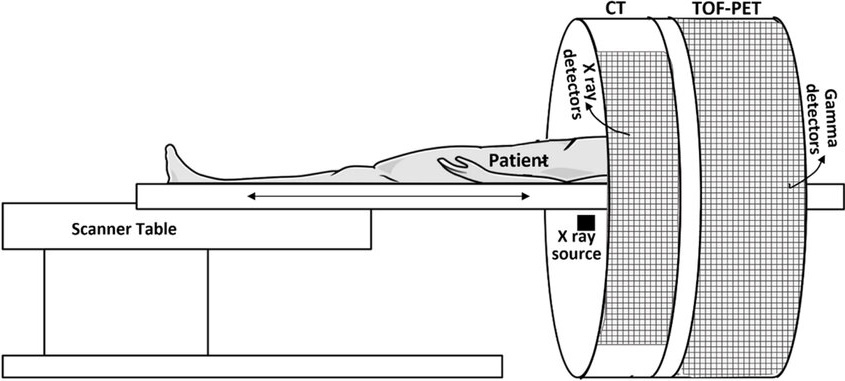
\includegraphics[width=0.45\textwidth]{assets/PETCTtable.jpg} 
	\caption{Schematic representation of TOF-capable PET/CT scanner with operational depiction of individual. Adapeted from Mohammadi \cite{figPETCT}}
	\label{fig:PETCTtable} 
\end{figure}

The device can be operatared separately or together within a single framework. In combined mode, CT images are employed for attenuation correction of PET data. When PET is used alone, it usually requieres for separate transmission scans used to provide anatomical reference and attenuation correction for images. Having them together improves imaging quaily while reducing examination time from additional scans \cite{townsend2004, zaidi2005}.

Clinical studies have demonstrated that even with shorter acquisition times, such as 1.5 minutes per bed position, image quality remains clinically acceptable with high rates of lesion visualization. PET/CT is a viable option for radiation workflows that are time-sensitive due to its efficiency and quality balance \cite{hasegawa2012}.


Modern PET/CT systems use advanced image registration techniques to improve data alignment and reduce errors.
Techniques for Deformable Image Registration (DIR), including GPU-accelerated DIR, take into consideration non-rigid changes brought on by patient movements or breathing patterns. 

Deformable Image Registration (DIR) methods such as, GPU-accelerated DIR, account for non-rigid transformations caused by patient motion or breathing patterns. These techniques model respiratory motion, improving the quantification and localization of functional uptake in PET imaging. In liver cancer treatment, where organ mobility presents major obstacles, such developments are very helpful \cite{shi2023}.

Additionally, this technique is considered upon its ability to detect non-FDG uptake lesions, contrasting with PET and helping avoid misdiagnosis in complex cases such as liver tumors \cite{yan2024, decazes2021}. This is done with segmentation algorithms that establish SUV thresholds to delineate lesions, integrating these volumes into treatment plans. Then, combining PET/CT with multiphasic CT can further characterize non-FDG lesions by leveraging dynamic contrast patterns visible in CT \cite{TG174}.

%\subsubsection{Dosimetry}
PET/CT is generally used for dosimetry calcuations, an example of this will be found on liver cancer treatments such as Yttrium-90 (\(^{90}\text{Y}\)) in the following section. Accurate dosimetry is dependent on quantitative imaging metrics such as standardized uptake values (SUVs). One of the advantages as explained in AAPMs TG174 and other papers is attenuation correction and faster acquisition times.\cite{knesaurek2018,TG174}. 

This system comes pre-integrated and aligns PET and CT datasets in the same frame of reference via software from the manufacturers and allows to acquire images in a single session ensuring precise alignment between functional and anatomical data.This reduces registration errors, ensuring precise tumor localization and dose delivery. 

CT imaging contributes with the electron density information necessary for attenuation correction in PET imaging. Since CT operates at lower photon energies (typically 80–140 keV), its data must be converted to match the 511 keV photons detected by PET. This calibration creates attenuation maps that align with PET imaging physics and are applied during PET image reconstruction to adjust the signal intensity, producing PET images that accurately represent metabolic activity without distortion due to tissue absorption.\cite{knesaurek2018, TG174}

In addition to attenuation correction, PET/CT facilitates tumor segmentation based on metabolic activity by converting PET data into standardized uptake values (SUVs). This information can then be integrated into radiotherapy planning systems to optimize treatment

Even with this seamless integration of the devices, respiratory motion and artifacts, particularly in liver cancer cases, can affect the accuracy of dose distribution. In TG174 we can find some techniques to mitigate respiratory motion artifacts in liver imaging as well as quality assurance (QA) protocols \cite{TG174}.

For example, TG174 highlights the use of respiratory gating to reduce motion artifacts caused by the liver’s movement during the breathing cycle. Or in the absence of respiratory gating, a time-weighted average intensity projection can mitigate the blurring effects of motion in PET intensity values.

Aside from this montly uniformity, quantification, and alignment tests between PET and CT datasets and annual Testing with phantoms, such as the ACR flangeless PET phantom, assesses PET/CT alignment and SUV accuracy are recomended.

Moreover, PET/CT tends to show lower SUV values compared to PET/MR, which may lead to underestimation of lesion uptake \cite{Prado-Wohlwend2023}. This underestimate can result in missed lesions, underestimation of disease severity, and incorrect staging of tumors. These limitations are particularly significant for liver imaging, where PET/MR has demonstrated increased diagnostic accuracy, with a 14.6\% improvement compared to PET/CT\cite{Prado-Wohlwend2023}.

In a case study, Knesaurek et al. \cite{knesaurek2018} reported differences in liver volume estimation between PET/CT and PET/MR, with a significant impact on dosimetry calculations. The discussion on this finding can be found on section \ref{sec:case}. This means that by choosing the correct imaging system for planing can make a huge difference. 


\subsection{PET/MR}
On the flip side, a relatively new imaging modality has been catching some interest, and could provide complementary benefits to PET/CT in radiotherapy. PET/Magnetic Resonance Imaging (PET/MR), while not as established as PET/CT can still provide soft-tissue contrast and functional imaging capabilities that are quite attractive for specific liver cancer cases.

This integration allows the recording of functional and anatomical information concurrently. The three prime strategies for combining PET/MR imaging include the following that are sequential, insert an integrated systems. In the systems that are sequential, there arrangement whereby a patient is allowed to be scanned first in pet scanner and subsequently in an MR-type scanner; this is easily enabled by having a prepared mechanical bed for moving the patient. This modality combination is easy but does not allow  simultaneous imaging. Misalignment and space are certainly an issue. In insert systems, a PET detector ring is inserted into the bore of an existing MR scanner. This approach allows simultaneous acquisition, superior spatial, and temporal alignment; however, several technical problems, such as magnetic field interference and limited bore size, make it suitable for rather specific applications, like neurological studies \cite{ziegler2013}.

Integrated PET/MR systems are defined as the direct integration of the PET detectors inside the MR scanner. Most common embodiments place the PET detector ring behind the radiofrequency coil of the MR scanner using a split superconducting magnet or field-cycled MR in order to be able to house the PET components. PET detectors in PET/MR systems are prepared by using materials that will not perturb the magnetic field and degrade the quality of MR images. Situating the detectors at the rear of the radiofrequency coil increases temperatures and may cause their oscillations. This is important because the gain of both APDs and SiPMs-commonly used in the construction of PET systems-depend on temperature \cite{ziegler2013,Muzic2014}. Schematics on each of these implamentations of the system are shown in figure \ref{fig:pet_mri_configurations}

\begin{figure}[H]
	\centering
	% Subfigure a: Sequential
	\begin{subfigure}[b]{0.45\textwidth}
		\centering
		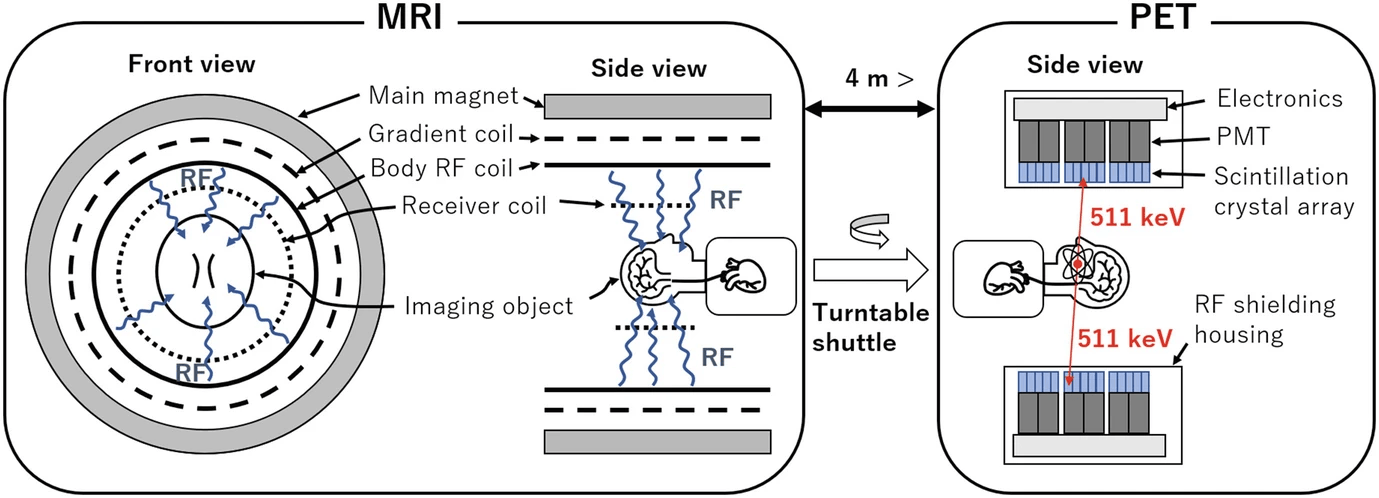
\includegraphics[width=\textwidth]{assets/sequencial.png}
		\caption{Sequential whole-body PET/MRI design using table shuttle for patient transportation.}
		\label{fig:sequential}
	\end{subfigure}
	% Subfigure b: Insert
	\begin{subfigure}[b]{0.45\textwidth}
		\centering
		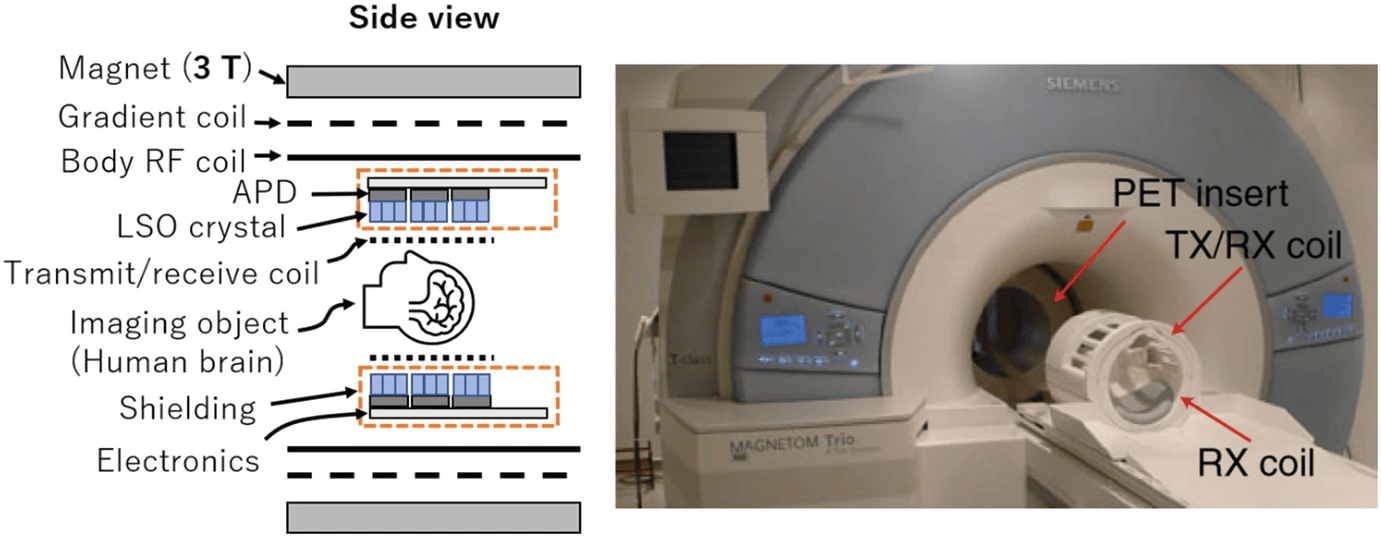
\includegraphics[width=\textwidth]{assets/insert.png}
		\caption{Schematic diagram of the APD-based brain PET insert with 3 T MRI and a photo of the brain PET insert combined with a slightly modified clinical 3 T MRI (right).}
		\label{fig:insert}
	\end{subfigure}
	
	% Subfigure c: Integrated
	\begin{subfigure}[b]{0.45\textwidth}
		\centering
		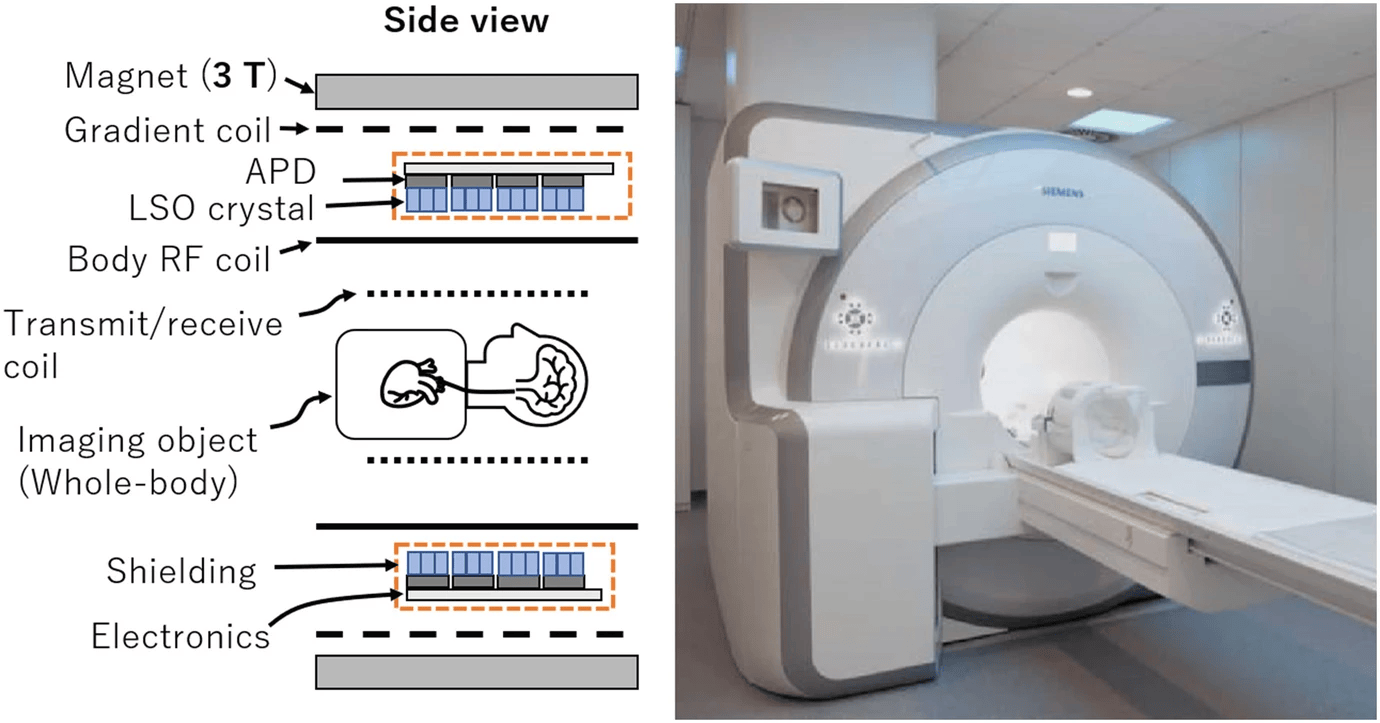
\includegraphics[width=\textwidth]{assets/integrated.png}
		\caption{Schematic diagram (left) and photo (right) of the first commercially available fully integrated whole-body PET/MR with APD technology.}
		\label{fig:integrated}
	\end{subfigure}
	
	\caption{Comparison of different PET/MRI configurations: (a) Sequential system, (b)Insert-based brain PET system. , and (c) Fully integrated system. Adapted from \cite{Kang2021}.}
	\label{fig:pet_mri_configurations}
\end{figure}


%\subsubsection{Soft Tissue Contrast}
Having better soft tissue contrast in the abdominal area aids the planning process by accurately delineating liver tumors from healthy tissue. Instead of relying on CT attenuation correction, MR benefits the patient with reduced radiation dose and better delineation of anatomical structures \cite{knesaurek2018}. This is really valuable for cases with small or poorly defined tumors.

Additionally, PET/MR’s ability to image respiratory liver motion during PET acquisition provides more reliable data for motion management compared to PET/CT \cite{knesaurek2018}. High-resolution MR images can also assist in partial volume corrections for PET images, further enhancing the precision of tumor targeting, but lacks electron density making attenuation correction challeging.

%\subsubsection{Functional Imaging}
PET by itself comes with functional data from the activity distribution, but MR will enhance this capabilities if combined with techniques like DWI (Diffusion-Weighted Imaging) and dynamic contrast-enhanced (DCE) imaging, for additional parameters on tumor metabolism and treatment response. 

\textbf{Diffusion-Weighted Imaging (DWI):} This technique assesses the movement of water molecules within tissues by measuring the Apparent Diffusion Coefficient (ADC). Tumors often exhibit lower ADC values due to high cellularity and restricted diffusion caused by cell membranes. Treatment-related changes in ADC values can reflect alterations in cellularity, serving as an early marker of therapeutic response \cite{pmc2010, ajr2006}.
\textbf{Dynamic Contrast-Enhanced (DCE) MRI:} DCE MRI tracks the distribution of contrast agents over time, providing valuable insights into blood flow and vascular integrity. Changes in perfusion patterns frequently correlate with treatment response, as increased perfusion often indicates effective therapy \cite{academic2021}.
Effective treatments typically lead to increased ADC values, reflecting reduced cellularity as tumor cells die. These changes can be observed within days to weeks after chemotherapy or radiotherapy. However, early treatment may cause transient decreases in ADC due to cellular swelling or vascular changes, necessitating careful interpretation \cite{pmc2010, pmc2009}.
Combining DCE MRI with PET data creates a multiparametric approach, integrating metabolic activity from PET with blood flow characteristics from DCE MRI. This synergy enhances the understanding of tumor behavior and supports personalized therapeutic strategies \cite{frontiers2020, springer2024}.

MR is already a solid tool for advance planning as explained in TG284\cite{TG284}. Despite these advantages, the longer acquisition times and lack of specific guidelines for PET/MR integration by AAPM make this technique rise questions. However, its use may be justified in cases where soft-tissue contrast is critical for treatment success. 

PET/MR contribute in a unique way to the planing and staging part, the following sections are to explore how this is implemented with radiation therapy and what is the overall effect on target delineation and dosimetry.



\subsection{PET/MR usage on Radiation Therapy}

%Yans Fig. 1 | Comparison of PET/MRI for radiotherapy procedures with conventional radiotherapy procedures
Figure \ref{fig:petmri_vs_conventional} shows the simplified workflow made possible by PET/MRI, compared to conventional radiotherapy procedures. According to Yan et al. \cite{yan2024}, PET/MRI greatly improves efficiency, eliminates the need for multiple devices, and minimizes mistakes from co-registration processes by integrating imaging and positioning steps into a single operation.

\end{multicols}

\begin{figure}[H]
\centering
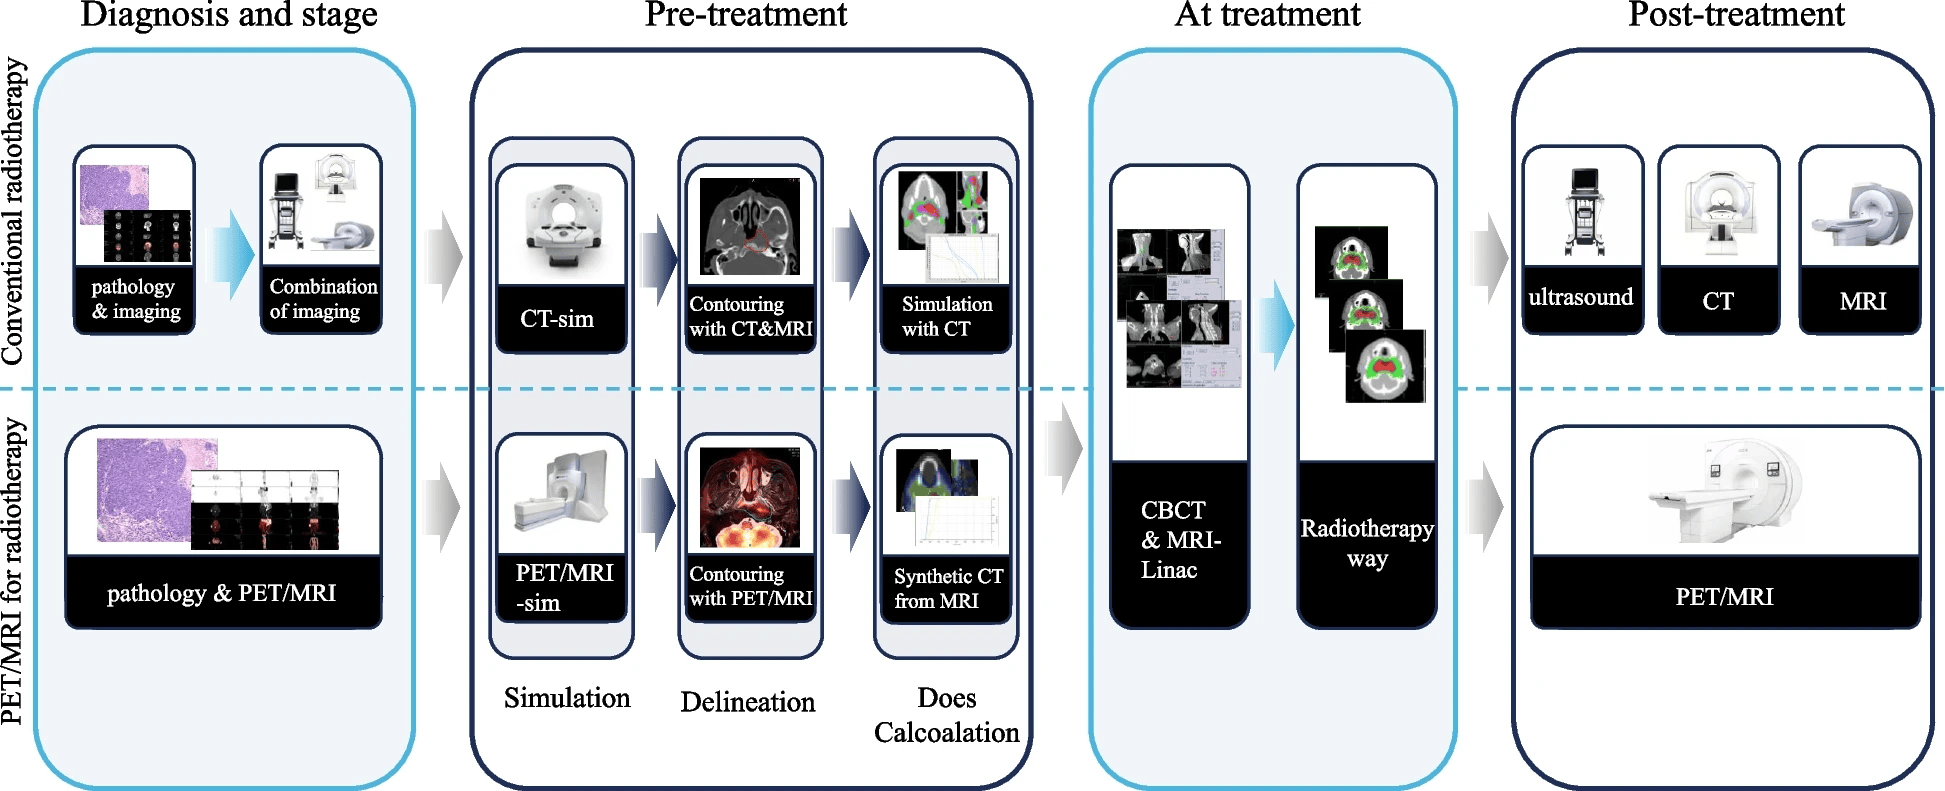
\includegraphics[width=1\textwidth]{assets/PETMRI_vs_Conventional_Workflow.png}
\caption{Comparison of PET/MRI workflows for radiotherapy procedures with conventional radiotherapy procedures. Adapted from Yan et al. \cite{yan2024}.}
\label{fig:petmri_vs_conventional}
\end{figure}%explain CBCT & MRI-Linac at treatment part


\begin{multicols}{2}

According to Decazes et al., adopting PET/MRI into radiation procedures needs careful planning and adjustments, that include using synthetic CT (pseudo-CT) for volume delineation and attenuation correction. %how would this be done
By immobilizing the patient, PET/MR allows for alignment between imaging modalities without the need for further registration procedures. In order to provide precise dosimetry planning without the need for several imaging devices, artificial intelligence methods, such GANs, further optimize attenuation mapping and shorten the pre-treatment routine \cite{decazes2021}.

%needs further explanation and development

\subsection{Positioning, Planning, and Pretreatment Workflow}

\paragraph{Specific Equipment and Material}
In order to properly use PET/MR in the clinical setting, challenges regarding patient positioning need to be addressed due to PET/MR's  %not yet described
unique design and functional requirements compared to PET/CT. The following discussion is primarily informed by Yan et al. \cite{yan2024}.%heavy reliance on one source
Regarding equipment, a regular curved diagnostic MR couch is unsuitable for PET. Instead, the use of flat treatment couch allows consistent patient positioning across imaging and treatment sessions while minimizing photon attenuation. Photon attenuation is further addressed in the materials used. Conventional carbon fiber tables, while minimally attenuating photons, can create surface currents that degrade MR image quality. Hybrid materials, such as plastic-foam sandwiches, have been developed to reduce photon attenuation and eliminate artifacts. Additionally, thin plastic shells and lightweight coil technologies are being explored to optimize attenuation correction (AC) without compromising image quality. \cite{yan2024, ziegler2013}

\paragraph{Effect on Image Quality}
The integration of these devices and materials influences the signal-to-noise ratio (SNR) and overall image quality. Phantom studies have shown negligible effects on SNR between flat and curved tables. However, positioning devices increase the distance between the patient and MR coils, reducing SNR by approximately 25\%. This reduction does not significantly impact target delineation accuracy. Techniques such as increasing the signal average, lowering acceleration factors, such as the reduction of parallel imaging acceleration, can also enhance SNR, or modifying echo times (e.g., by optimizing the echo spacing for a given tissue type) can improve image contrast and mitigate SNR loss, though these adjustments may increase acquisition time. \cite{yan2024,Rostami2024}

\paragraph{Attenuation Correction}
Due to the lack of CT in these devices, attenuation correction is a major challenge. For example, rigid hardware such as coil holders and flat tables are usually accounted for using CT-based 3D AC maps or isotope-based attenuation maps; this is no longer the case for PET/MR. There is a need to introduce coil fixation devices that mitigate errors caused by the variable positioning of flexible RF coils during scanning to improve reliability of AC maps. Moreover, there is a bone segmentation limitation. MR-based AC often excludes bone due to the low intensity of bone signals in MR images. Atlas-based methods, which use pre-existing templates of CT anatomy to generate a pseudo-CT for attenuation correction, can incorporate bone structures but may introduce registration errors in regions with varying stiffness, such as the abdomen.

Overall, consistent positioning is critical to ensure reliable imaging and proper AC. Studies using phantoms have demonstrated minimal deviations in accuracy during multiple repositioning with RF coil holders. Additionally, PET/MR simulator tables allow single registration for fixed tabletop setups, ensuring repeatability in radiation therapy workflows.

\paragraph{Target delineation}
Tumor delineation in radiotherapy involves the definition of at least 3 different volumes, gross tumor volume (GTV), clinical target volume (CTV), and planning target volume (PTV). PET/MR offers unique advantages over conventional imaging modalities, particularly in refining GTV boundaries by integrating both morphological and biological data.


MRI alone is commonly used to outline the GTV based on tumor morphology, while PET provides additional biological insights that mitigate the risk of marginal misses. Studies cited in Yan et al. demonstrate Zhang et al.’s \cite{Zhang2014} observation that PET imaging contributed to an approximate 10\% increase in tumor volume detection not captured by MRI alone.\cite{yan2024} This finding better explains tumor sizes measured under a microscope, it is also supported by comparisons of Dice Similarity Coefficient (DSC), a metric used to assess the overlap between imaging-based tumor delineations and the ground truth, he explains.%who? i think Zhang

This difference on the outline of the GTV is shown in figure \ref{fig:gtv_delineation_cropped}, while it focuses on nasopharyngeal cancer, it provides valuable insights into the comparative performance of PET/MRI and PET/CT for tumor delineation. Soft-tissue contrast of PET/MRI is especially relevant for complex tumor regions, such as the liver.

%Yans Fig. 3 | Nasopharyngeal GTV delineations across modalities

%	•	Highly relevant to tumor delineation discussions but less so for liver cancer.
%	•	Acknowledge that it focuses on nasopharyngeal cancer while emphasizing generalizable findings.


\begin{figure}[H]
	\centering
	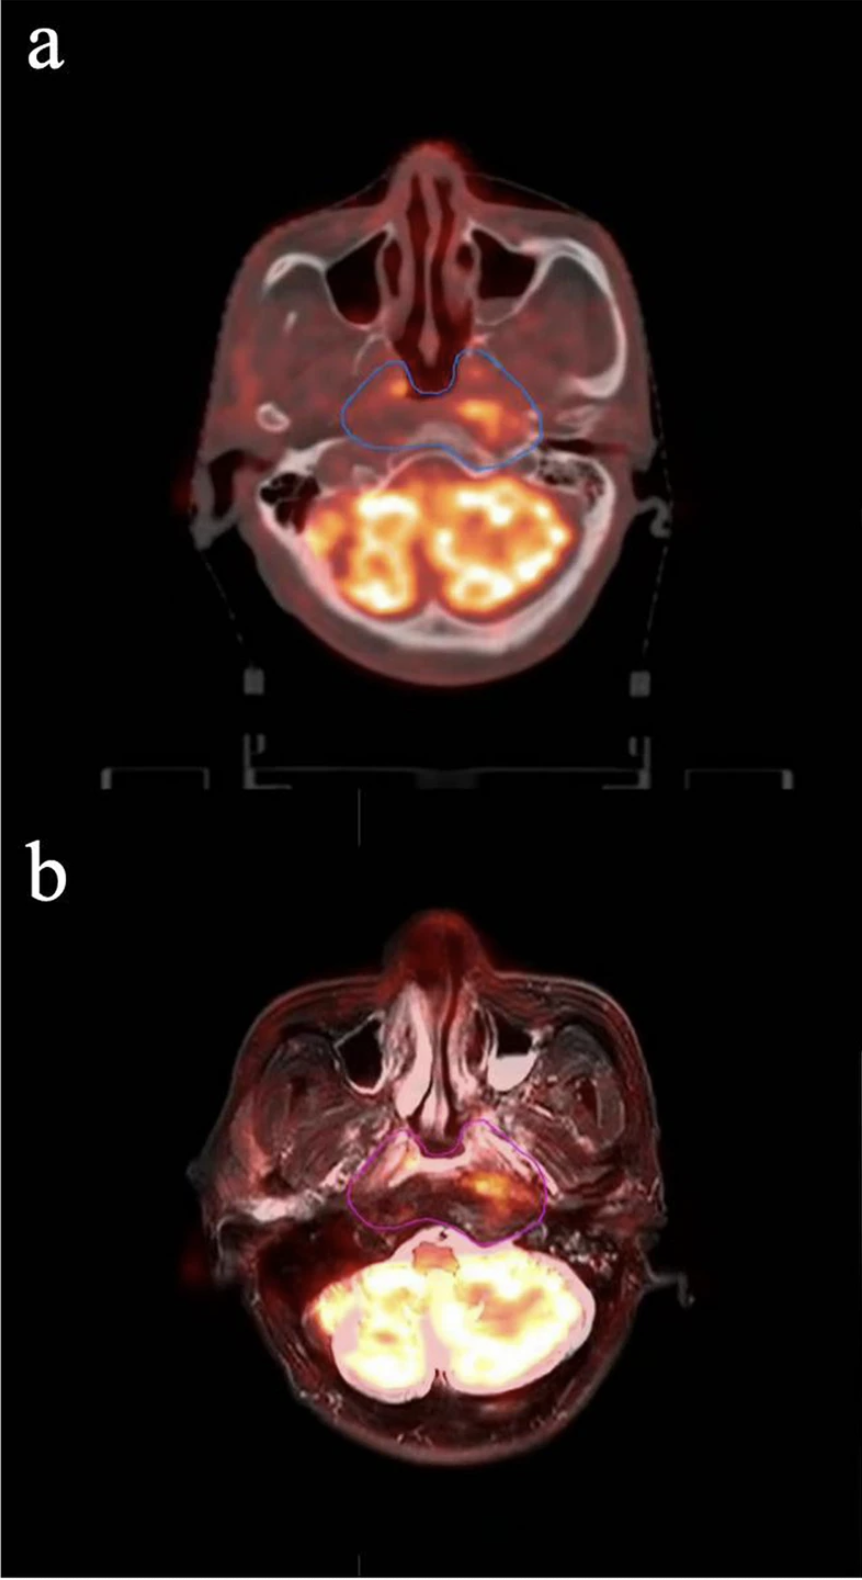
\includegraphics[width=0.8\columnwidth]{assets/GTV_Delineation_PETCT_vs_PETMRI.png} 
	\caption{Gross tumor volume (GTV) delineation across PET/CT and PET/MRI modalities for a 69-year-old female with nasopharynx cancer. (a) The blue line represents GTV-PET/CT. (b) The pink line represents GTV-PET/MRI. Adapted from Yan et al. \cite{yan2024}.}
	\label{fig:gtv_delineation_cropped}
\end{figure}

The addition of PET provides some advantages as well, PET’s ability to capture tumor biology introduces the concept of Biological Target Volume (BTV), which integrates metabolic and functional characteristics of tumors. Using BTV data, radiotherapy can deliver higher doses to treatment-resistant regions while sparing sensitive areas. This approach, known as "dose painting" or "dose sculpting," aims to increase cure rates without increasing late radiation-induced toxicity. \cite{Schinagl2006}

Of course there are limitations, starting from manual tumor delineation, though widely used, it introduces significant variability. To address this, adaptive thresholding based on individual standardized uptake values (SUVmax) and automated delineation methods are being explored. For example, PET/MRI’s co-segmentation methods have been shown to match observer performance in target delineation while providing more consistent results across repeated evaluations \cite{yan2024}. And regarding its comparison to PET/CT, PET/MR has reduced SUVmax values that may lead to conservative tumor boundaries.

The integration of PET in radiotherapy planning has led to significant alterations in radiation treatment volumes for 30\%-60\% of non-small cell lung cancer (NSCLC) patients. \cite{Bradley2004}. PET/CT has improved stereotactic body radiation therapy (SBRT) treatment in NSCLC patients by advancing the development of prognostic PET/CT radiomic signatures \cite{Vijayakumar2022}.

\paragraph{Dose Calculation and Optimization}

Once the target volume is delineated, the next step of planing is dose calculations. For PET/MR there are technical considerations compared to PET/CT, particularly in the context of SBRT, where precision in dose distribution is everything.

The main challenge presented on PET/MR is that it lacks the capability to directly acquire tissue electron density values. As of right now workflows include co-register PET/MR with CT images to generate dose prescription maps. Studies found that pseudo-CT techniques generated from MR images have high accuracy, and reported negligible mean absolute errors of 0.17 ± 0.12 Gy in dosimetry analysis \cite{yan2024}.

However, PET/MR offers significant advantages for SBRT planning, particularly in reducing radiation exposure. Time-of-Flight (TOF) PET/MR systems require only 35\% of the activity concentration needed for TOF-PET/CT while maintaining comparable image quality, translating to a theoretical dose reduction of up to 65\%, with clinical observations suggesting realistic reductions exceeding 50\% \cite{Queiroz2015,Polan2023}. 

\subsubsection{Mid-Treatment Workflow}

In accordance with Yan et al., [18F]-FDG PET/MRI mid-treatment assessments offer essential details on tumor response using metrics that include $\Delta \text{SUVmax}$ and $\Delta \text{Dmin}$. Their function is to provide predictions for treatment sensitivity and risk of recurrence. Significant changes in water transport and glucose metabolism were noted throughout treatment, allowing for adaptive therapy modification to prevent toxicity or accelerated tumor development \cite{yan2024}.  

A way to take advantage from this preparation, incorporating PET-based absorbed dose map into mid-treatment workflows for SBRT or SIRT is possible. Polan et al. (2023) studied how sequentially integrating $^{90}\text{Y}$-PET-based dose distribution clinicians were able to refine treatment plans, enhancing the precision of dose delivery and adapting to dynamic tumor changes during therapy \cite{Polan2023}. 

Addditionally, studies have shown that  advanced techniques, such as Intensity-Modulated Radiation Therapy (IMRT) and Volumetric Modulated Arc Therapy (VMAT), particularly benefit from advanced imaging techniques by leverage real-time anatomical and functional imaging to adjust dose distributions dynamically \cite{Hunte2022,Tsang2016}.

Referencing back to Figure \ref{fig:petmri_vs_conventional}, after using PET/MR and synthetic CT to performe treatment planing and dosimetric calculations, Cone-Beam Computed Tomography (CBCT) and MRI-guided Linear Accelerators (MRI-LINAC) are suggested for mid treatment assesment. CBCT provides high-resolution imaging of anatomical structures, enabling precise verification of patient positioning and tumor morphology before and during treatment. By capturing volumetric data, CBCT facilitates precise target localization and minimizes setup uncertainties, a key requirement for the high precision demanded in SBRT \cite{Srinivasan2014}.

MRI-LINAC, on the other hand, combines the superior soft-tissue contrast of MRI with real-time radiation delivery. This integration allows clinicians to continuously monitor tumors and surrounding tissues with unparalleled clarity, enabling dynamic adjustments during treatment. They also are methodologies for adaptative therapy workflows. For SBRT, sub-millimeter precision is critical,  and MRI-LINAC ensures that the radiation dose is confined to the target while sparing adjacent organs at risk. The ability to visualize and adapt to changes in tumor size, shape, and position during therapy enhances the precision and safety of treatments. Furthermore, MRI-LINAC supports adaptive planning workflows, as demonstrated by Lei et al. (2020) and Cunningham et al. (2022), where the incorporation of synthetic MRI and cine MRI imaging techniques have significantly improved tumor tracking and dose conformity in SBRT \cite{Lei2020,Cunningham2022}.
\end{multicols}